\subparagraph*{Problem explaination}
The goal is the same of the previous problem, but in this case the conversion rates are not stationary and is required to use a sliding-window approach.
\subparagraph*{Strategy}
In a non-stationary environment the conversion rates are not stationary, so they change due to the seasonalities.
We exploit the sliding-window approach combined with the Thompson sampling algorithm (SW-TS) to solve this problem. It is an algorithm that exploits a Sliding-Window approach to forget past information  during the learning, which could provide a bias to the estimation process.
\subparagraph*{Sliding-Window Thompson Sampling (SW-TS)} 

\textbf{Main idea:}\\
We use a sliding window of length $\tau\in N$ such that the algorithm, at every round $t$, takes into account only the rewards obtained in the last $\tau$ rounds. Based on these realizations, we apply a TS-based algorithm to decide which is the arm to pull in the next round. In particular, the expected value of each arm is coupled with a posterior distribution from which we draw samples, and the arm with the highest value is the next arm to play.\\

\textbf{Pseudocode:}\\

1. At every time $t$ for every arm $a$:

$\tilde{\theta_{a}} \leftarrow Sample(\mathbb P(\mu_{a}=\theta_{a}))$ \\

2. At every time $t$ play arm $a_{t}$ such that 

$a_{t} \leftarrow \argmax_{a \in A} \left\{ \tilde{\theta_{a}}  \right\} $ \\

3.  Update beta distribution of arm $a_{t}$

if $t\leq\tau$: $(\alpha_{a_{t}}, \beta_{a_{t}}) \leftarrow (\alpha_{a_{t}}, \beta_{a_{t}}) + (x_{a_{t},t}, 1 - x_{a_{t},t})$ 

if $\tau<t$:	$(\alpha_{a_{t}}, \beta_{a_{t}}) \leftarrow \max \left\{(1,1), (\alpha_{a_{t}}, \beta_{a_{t}}) + (x_{a_{t},t}, 1 - x_{a_{t},t}) - (x_{a_{t-\tau},t-\tau}, 1 - x_{a_{t-\tau},t-\tau})    \right\}$
\subparagraph*{Results}
\begin{center}
	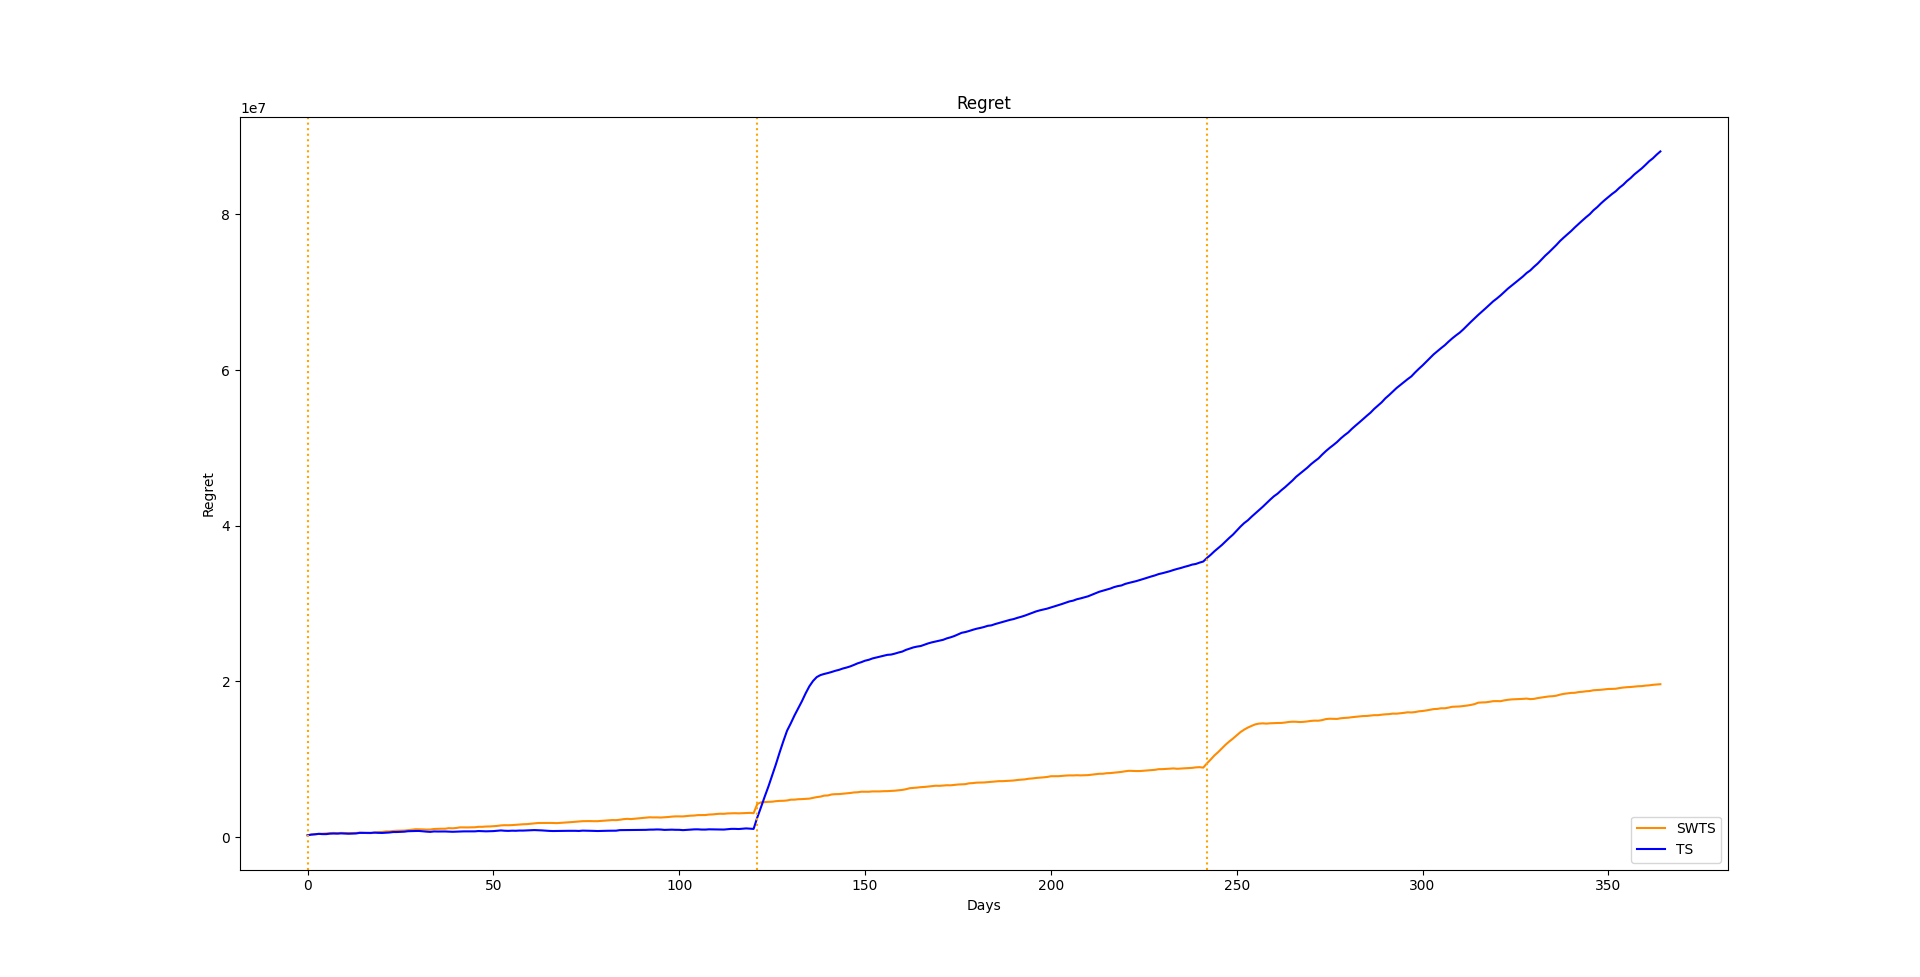
\includegraphics[scale=0.30]{Images/n7}
\end{center}
\subparagraph*{Considerations}
We can observe that in the first season the SW-TS algorithm has an higher regret than the TS algorithm, because the first has a number of samples that is equal to the dimension of the window, instead the second collects all the samples. The SW-TS has a better performance from the second season, due to the sliding-window approach, it stabilizes faster than the TS, and at the end, the cumulative regret for the SW-TS is about 4 times less than the TS.